\documentclass[]{article}
\usepackage[a4paper, total={15cm,23cm}]{geometry}
\usepackage{fancyhdr}
\usepackage{graphicx}
\usepackage{amsmath}
\usepackage{amssymb}
\usepackage{xcolor}
\usepackage{tikz}
\usepackage{verbatim}
\usepackage{tcolorbox}
\usepackage{textcomp}
\usepackage{xcomment}
\usepackage{xstring}
\usepackage{array}
%opening
\title{PH 223 Week 9}
\author{Benjamin Bauml and Danielle Skinner}
\date{Winter 2024}
\pagestyle{fancy}
\rhead{PH 223}
\chead{Winter 2024}
\lhead{Week 9}

% Version 2024-02-21
% Changes
% 2024-02-21 Added xstring package to enable smooth implementation of new \ModePage command.
% For Assignment, leave Purpose as 1. For Worksheet, set to 2. For Student Solution, set to 3. For Teacher Solution, set to 4.
\newcommand{\Purpose}{1}

\newcommand{\Exclusion}{0}
\newcommand{\PageTurn}{0}
\newcommand{\GrayProb}{0}
\newcommand{\Tipsy}{0}

% Assignment
\if\Purpose1
\renewcommand{\Exclusion}{1}
\fi
% Worksheet
\if\Purpose2
\renewcommand{\Exclusion}{1}
\renewcommand{\PageTurn}{1}
\fi
% Student Solution
\if\Purpose3
\renewcommand{\PageTurn}{1}
\renewcommand{\GrayProb}{1}
\fi
% Teaching Copy
\if\Purpose4
\renewcommand{\PageTurn}{1}
\renewcommand{\GrayProb}{1}
\renewcommand{\Tipsy}{1}
\fi

\if\Exclusion1
\xcomment{Title,Problem,ProblemSub,PassFig}
\fi

\def \NewQ {0}
\def \PForce {0}
\newcommand{\MaybePage}[1]{
	\def \PForce {#1}
	\if\PForce1
		\newpage
	\else
		\if\NewQ0
		\gdef \NewQ {\PageTurn}
		\else
		\newpage
		\fi
	\fi
}

\newcommand{\ModePage}[1]{
	\IfSubStr{#1}{\Purpose}{\newpage}{}
}

\newenvironment{Problem}[2][0]{%The first argument is optional, and if it is set to 1, the \newpage will be forced.
\MaybePage{#1}
\section*{#2}
\if\GrayProb1
\begin{tcolorbox}[colback=lightgray,colframe=lightgray,sharp corners,boxsep=1pt,left=0pt,right=0pt,top=0pt,bottom=0pt,after skip=2pt]
\else
\begin{tcolorbox}[colback=white,colframe=white,sharp corners,boxsep=1pt,left=0pt,right=0pt,top=0pt,bottom=0pt,after skip=2pt]
\fi
}{
\end{tcolorbox}\noindent
}

\newenvironment{ProblemSub}[1][0]{%The argument is optional, and if a string of numbers is entered into it, it will force a \newpage in any \Purpose that shows up in the string. For example, "13" would lead to the newpage being forced in modes 1 and 3.
\ModePage{#1}
\if\GrayProb1
\begin{tcolorbox}[colback=lightgray,colframe=lightgray,sharp corners,boxsep=1pt,left=0pt,right=0pt,top=0pt,bottom=0pt,after skip=2pt]
\else
\begin{tcolorbox}[colback=white,colframe=white,sharp corners,boxsep=1pt,left=0pt,right=0pt,top=0pt,bottom=0pt,after skip=2pt]
\fi
}{
\end{tcolorbox}\noindent
}

\newenvironment{PassFig}{\begin{figure}[h]}{\end{figure}}

\newcommand{\TeachingTips}[1]{
\if\Tipsy1
\begin{tcolorbox}[colback=lightgray,colframe=black]
#1
\end{tcolorbox}
\fi
}

\newenvironment{Title}{\maketitle}{}

\begin{document}
\begin{Title}
\begin{center}
	The first two problems are borrowed/adapted from Chapters 29 and 30 of the \textit{Student Workbook} for \textit{Physics for Scientists and Engineers}.
\end{center}
\end{Title}

\begin{Problem}{Activity 1}
	A metal wire is resting on a U-shaped conducting rail. The rail is fixed in position, but the wire is free to move.
\end{Problem}
\begin{ProblemSub}
	(a) If the magnetic field is increasing in strength, does the wire:
\end{ProblemSub}
\begin{PassFig}
	\centering
	\if\GrayProb1
		\includegraphics[scale=0.7]{A2Sol}
	\else
		\includegraphics[scale=0.7]{A2}
	\fi
\end{PassFig}
\begin{ProblemSub}
	Explain your choice.
\end{ProblemSub}
The wire moves to the left. The downward flux is increasing. To oppose this increase, an induced field must point up, which requires a counterclockwise current (i.e. up on the wire). Using $ I\vec{l}\times\vec{B} $ gives a force that pulls the wire to the left.
\begin{ProblemSub}
	(b) If the magnetic field is decreasing in strength, which of the above happens? Explain.
\end{ProblemSub}
The wire moves to the right. Now, the downward flux is decreasing, so the induced current will be clockwise (i.e. down the wire). The force $ I\vec{l}\times\vec{B} $ will pull the wire to the right.

\begin{Problem}[1]{Activity 2}
	The magnetic field above the dotted line is $ \vec{B} = (2\text{ T, right}) $. Below the dotted line, the field is $ \vec{B} = (2\text{ T, left}) $. Each closed loop is 1 m $ \times $ 1 m.
\end{Problem}
\begin{PassFig}
	\centering
	\includegraphics[scale=0.8]{A2-8}
\end{PassFig}
\begin{ProblemSub}
	(a) Let's evaluate the line integral of $ \vec{B} $ around each of these closed loops by breaking the integration into four steps. We'll go around the loop in a \textit{clockwise} direction. Pay careful attention to signs.
\end{ProblemSub}
\begin{PassFig}
	\centering
	\if\GrayProb1
	\includegraphics[scale=0.9]{A2aSol}
	\else
	\includegraphics[scale=0.9]{A2a}
	\fi
\end{PassFig}
\begin{ProblemSub}
	(b) What is the current through loop 2, and what direction is it in?
\end{ProblemSub}
By Amp\`{e}re's law, $ \oint\vec{B}\cdot d\vec{s} = \mu_{0}I_{enc} $. We know that $ \oint\vec{B}\cdot d\vec{s} = 4 $ T$ \cdot $m in loop 2, so $ I_{enc} = \frac{4\text{ T}\cdot\text{m}}{\mu_{0}} $. This current points into the page, as the clockwise orientation of our loop points its surface normal into the page. This field is what one might expect from an infinite plane of surface current $ \vec{K} = (4\text{ T}/\mu_{0}\text{, into the page}) $.

\begin{Problem}{Activity 3: Induction Table}
	(a) For each case below, fill out the table with the corresponding information. If the quantity is a vector, draw an arrow indicating the direction of the vector. If it is a scalar, indicate the sign of the scalar with a $+$, $-$, or 0. Remember that $\vec{\mu} = I\vec{A}$.
	
	On the loops, draw the up area vector in red and the down area vector in black. When you determine the current for each area vector, draw the direction of the current on the loop with the corresponding color. Case A has been completed as an example.
\end{Problem}
\begin{PassFig}
	\centering
	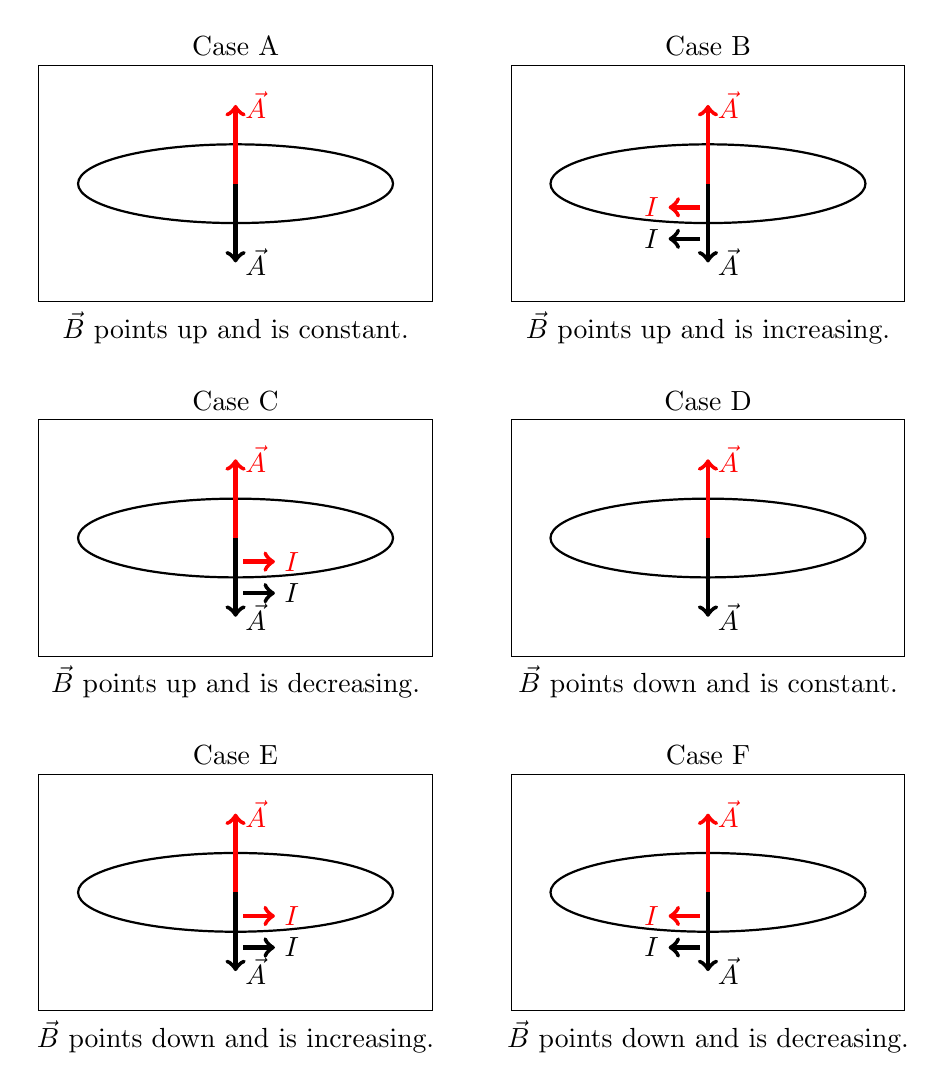
\begin{tikzpicture}
		\begin{scope}[shift={(-3cm,0)}]
			\node[anchor=south] at (0,1.5cm) {Case A};
			\draw (-2.5cm,1.5cm) -- (2.5cm,1.5cm) -- (2.5cm,-1.5cm) -- (-2.5cm,-1.5cm) -- cycle;
			\draw[ultra thick,->] (0,0) -- (0,-1cm);
			\node[anchor=west] at (0,-1cm) {$\vec{A}$};
			\draw[thick] (0,0) ellipse (2cm and 0.5cm);
			\draw[ultra thick,red,->] (0,0) -- (0,1cm);
			\node[anchor=west] at (0,1cm) {\color{red}$\vec{A}$};
			\node[anchor=north] at (0,-1.5cm) {$\vec{B}$ points up and is constant.};
		\end{scope}
		\begin{scope}[shift={(3cm,0)}]
			\node[anchor=south] at (0,1.5cm) {Case B};
			\draw (-2.5cm,1.5cm) -- (2.5cm,1.5cm) -- (2.5cm,-1.5cm) -- (-2.5cm,-1.5cm) -- cycle;
			\if\GrayProb1
			\draw[ultra thick,->] (0,0) -- (0,-1cm);
			\node[anchor=west] at (0,-1cm) {$\vec{A}$};
			\draw[ultra thick,->] (-0.1cm,-0.7cm) -- (-0.5cm,-0.7cm);
			\node[anchor=east] at (-0.5cm,-0.7cm) {$I$};
			\fi
			\draw[thick] (0,0) ellipse (2cm and 0.5cm);
			\if\GrayProb1
			\draw[ultra thick,red,->] (0,0) -- (0,1cm);
			\node[anchor=west] at (0,1cm) {\color{red}$\vec{A}$};
			\draw[ultra thick,red,->] (-0.1cm,-0.3cm) -- (-0.5cm,-0.3cm);
			\node[anchor=east] at (-0.5cm,-0.3cm) {\color{red}$I$};
			\fi
			\node[anchor=north] at (0,-1.5cm) {$\vec{B}$ points up and is increasing.};
		\end{scope}
		\begin{scope}[shift={(-3cm,-4.5cm)}]
			\node[anchor=south] at (0,1.5cm) {Case C};
			\draw (-2.5cm,1.5cm) -- (2.5cm,1.5cm) -- (2.5cm,-1.5cm) -- (-2.5cm,-1.5cm) -- cycle;
			\if\GrayProb1
			\draw[ultra thick,->] (0,0) -- (0,-1cm);
			\node[anchor=west] at (0,-1cm) {$\vec{A}$};
			\draw[ultra thick,->] (0.1cm,-0.7cm) -- (0.5cm,-0.7cm);
			\node[anchor=west] at (0.5cm,-0.7cm) {$I$};
			\fi
			\draw[thick] (0,0) ellipse (2cm and 0.5cm);
			\if\GrayProb1
			\draw[ultra thick,red,->] (0,0) -- (0,1cm);
			\node[anchor=west] at (0,1cm) {\color{red}$\vec{A}$};
			\draw[ultra thick,red,->] (0.1cm,-0.3cm) -- (0.5cm,-0.3cm);
			\node[anchor=west] at (0.5cm,-0.3cm) {\color{red}$I$};
			\fi
			\node[anchor=north] at (0,-1.5cm) {$\vec{B}$ points up and is decreasing.};
		\end{scope}
		\begin{scope}[shift={(3cm,-4.5cm)}]
			\node[anchor=south] at (0,1.5cm) {Case D};
			\draw (-2.5cm,1.5cm) -- (2.5cm,1.5cm) -- (2.5cm,-1.5cm) -- (-2.5cm,-1.5cm) -- cycle;
			\if\GrayProb1
			\draw[ultra thick,->] (0,0) -- (0,-1cm);
			\node[anchor=west] at (0,-1cm) {$\vec{A}$};
			\fi
			\draw[thick] (0,0) ellipse (2cm and 0.5cm);
			\if\GrayProb1
			\draw[ultra thick,red,->] (0,0) -- (0,1cm);
			\node[anchor=west] at (0,1cm) {\color{red}$\vec{A}$};
			\fi
			\node[anchor=north] at (0,-1.5cm) {$\vec{B}$ points down and is constant.};
		\end{scope}
		\begin{scope}[shift={(-3cm,-9cm)}]
			\node[anchor=south] at (0,1.5cm) {Case E};
			\draw (-2.5cm,1.5cm) -- (2.5cm,1.5cm) -- (2.5cm,-1.5cm) -- (-2.5cm,-1.5cm) -- cycle;
			\if\GrayProb1
			\draw[ultra thick,->] (0,0) -- (0,-1cm);
			\node[anchor=west] at (0,-1cm) {$\vec{A}$};
			\draw[ultra thick,->] (0.1cm,-0.7cm) -- (0.5cm,-0.7cm);
			\node[anchor=west] at (0.5cm,-0.7cm) {$I$};
			\fi
			\draw[thick] (0,0) ellipse (2cm and 0.5cm);
			\if\GrayProb1
			\draw[ultra thick,red,->] (0,0) -- (0,1cm);
			\node[anchor=west] at (0,1cm) {\color{red}$\vec{A}$};
			\draw[ultra thick,red,->] (0.1cm,-0.3cm) -- (0.5cm,-0.3cm);
			\node[anchor=west] at (0.5cm,-0.3cm) {\color{red}$I$};
			\fi
			\node[anchor=north] at (0,-1.5cm) {$\vec{B}$ points down and is increasing.};
		\end{scope}
		\begin{scope}[shift={(3cm,-9cm)}]
			\node[anchor=south] at (0,1.5cm) {Case F};
			\draw (-2.5cm,1.5cm) -- (2.5cm,1.5cm) -- (2.5cm,-1.5cm) -- (-2.5cm,-1.5cm) -- cycle;
			\if\GrayProb1
			\draw[ultra thick,->] (0,0) -- (0,-1cm);
			\node[anchor=west] at (0,-1cm) {$\vec{A}$};
			\draw[ultra thick,->] (-0.1cm,-0.7cm) -- (-0.5cm,-0.7cm);
			\node[anchor=east] at (-0.5cm,-0.7cm) {$I$};
			\fi
			\draw[thick] (0,0) ellipse (2cm and 0.5cm);
			\if\GrayProb1
			\draw[ultra thick,red,->] (0,0) -- (0,1cm);
			\node[anchor=west] at (0,1cm) {\color{red}$\vec{A}$};
			\draw[ultra thick,red,->] (-0.1cm,-0.3cm) -- (-0.5cm,-0.3cm);
			\node[anchor=east] at (-0.5cm,-0.3cm) {\color{red}$I$};
			\fi
			\node[anchor=north] at (0,-1.5cm) {$\vec{B}$ points down and is decreasing.};
		\end{scope}
	\end{tikzpicture}
\end{PassFig}
\begin{PassFig}
	\centering
	\if\GrayProb1
	\begin{tabular}{|c||>{\centering\arraybackslash}m{0.3cm}|>{\centering\arraybackslash}m{0.3cm}||>{\centering\arraybackslash}m{0.3cm}|>{\centering\arraybackslash}m{0.3cm}||>{\centering\arraybackslash}m{0.3cm}|>{\centering\arraybackslash}m{0.3cm}||>{\centering\arraybackslash}m{0.3cm}|>{\centering\arraybackslash}m{0.3cm}||>{\centering\arraybackslash}m{0.3cm}|>{\centering\arraybackslash}m{0.3cm}||>{\centering\arraybackslash}m{0.3cm}|>{\centering\arraybackslash}m{0.3cm}|}
		\hline
		\multicolumn{1}{|c||}{} & \multicolumn{2}{c||}{Case A} & \multicolumn{2}{c||}{Case B} & \multicolumn{2}{c||}{Case C} & \multicolumn{2}{c||}{Case D} & \multicolumn{2}{c||}{Case E} & \multicolumn{2}{c|}{Case F} \\
		\hline
		\hline
		$\vec{A}$ & {\color{red}$\uparrow$} & $\downarrow$ & {\color{red}$\uparrow$} & $\downarrow$ & {\color{red}$\uparrow$} & $\downarrow$ & {\color{red}$\uparrow$} & $\downarrow$ & {\color{red}$\uparrow$} & $\downarrow$ & {\color{red}$\uparrow$} & $\downarrow$ \\
		\hline
		$\vec{B}$ & $\uparrow$ & $\uparrow$ & $\uparrow$ & $\uparrow$ & $\uparrow$ & $\uparrow$ & $\downarrow$ & $\downarrow$ & $\downarrow$ & $\downarrow$ & $\downarrow$ & $\downarrow$ \\
		\hline
		$\Phi_{B}$ & $+$ & $-$ & $+$ & $-$ & $+$ & $-$ & $-$ & $+$ & $-$ & $+$ & $-$ & $+$ \\
		\hline
		$\frac{d\Phi_{B}}{dt}$ & $0$ & $0$ & $+$ & $-$ & $-$ & $+$ & $0$ & $0$ & $-$ & $+$ & $+$ & $-$ \\
		\hline
		$V_{ind}$ & $0$ & $0$ & $-$ & $+$ & $+$ & $-$ & $0$ & $0$ & $+$ & $-$ & $-$ & $+$ \\
		\hline
		$I_{ind}$ & $0$ & $0$ & $-$ & $+$ & $+$ & $-$ & $0$ & $0$ & $+$ & $-$ & $-$ & $+$ \\
		\hline
		$\vec{\mu}$ & $0$ & $0$ & $\downarrow$ & $\downarrow$ & $\uparrow$ & $\uparrow$ & $0$ & $0$ & $\uparrow$ & $\uparrow$ & $\downarrow$ & $\downarrow$ \\
		\hline
	\end{tabular}
	\else
	\begin{tabular}{|c||>{\centering\arraybackslash}m{0.3cm}|>{\centering\arraybackslash}m{0.3cm}||>{\centering\arraybackslash}m{0.3cm}|>{\centering\arraybackslash}m{0.3cm}||>{\centering\arraybackslash}m{0.3cm}|>{\centering\arraybackslash}m{0.3cm}||>{\centering\arraybackslash}m{0.3cm}|>{\centering\arraybackslash}m{0.3cm}||>{\centering\arraybackslash}m{0.3cm}|>{\centering\arraybackslash}m{0.3cm}||>{\centering\arraybackslash}m{0.3cm}|>{\centering\arraybackslash}m{0.3cm}|}
		\hline
		\multicolumn{1}{|c||}{} & \multicolumn{2}{c||}{Case A} & \multicolumn{2}{c||}{Case B} & \multicolumn{2}{c||}{Case C} & \multicolumn{2}{c||}{Case D} & \multicolumn{2}{c||}{Case E} & \multicolumn{2}{c|}{Case F} \\
		\hline
		\hline
		$\vec{A}$ & {\color{red}$\uparrow$} & $\downarrow$ &  &  &  &  &  &  &  &  &  &  \\
		\hline
		$\vec{B}$ & $\uparrow$ & $\uparrow$ &  &  &  &  &  &  &  &  &  &  \\
		\hline
		$\Phi_{B}$ & $+$ & $-$ &  &  &  &  &  &  &  &  &  &  \\
		\hline
		$\frac{d\Phi_{B}}{dt}$ & $0$ & $0$ &  &  &  &  &  &  &  &  &  &  \\
		\hline
		$V_{ind}$ & $0$ & $0$ &  &  &  &  &  &  &  &  &  &  \\
		\hline
		$I_{ind}$ & $0$ & $0$ &  &  &  &  &  &  &  &  &  &  \\
		\hline
		$\vec{\mu}$ & $0$ & $0$ &  &  &  &  &  &  &  &  &  &  \\
		\hline
	\end{tabular}
	\fi
\end{PassFig}

Note that when the magnetic field is increasing (as in Case B), the flux can still be decreasing, as its sign depends on your choice of area vector. If the area vector is down, then the flux in Case B is negative, and the increasing magnetic field means the flux gets more negative (decreases) over time.
\begin{ProblemSub}[2]
	(b) Does your choice of area vector change the final answer?
\end{ProblemSub}
The area vector is an imaginary mathematical object that helps us orient the problem and establish sign conventions. It may affect the signs of certain other mathematical quantities, but observable properties of the loop cannot be different. As we can see, the direction of current flow and magnetic moment are the same no matter which area vector is chosen. Positive current just means that it flows counterclockwise around the area vector, so positive current around an upward area vector is the same as negative current around a downward area vector. The negative current, when multiplied by the area vector, reverses its direction to keep the direction of $\vec{\mu}$ consistent.
\begin{ProblemSub}
	(c) How is the direction of $\vec{\mu}$ related to the direction of the change in the external magnetic field?
\end{ProblemSub}
Note that $\vec{\mu}$ points opposite the external magnetic field when the external field is increasing, and it points in the same direction as the external field when the external field is decreasing. The current induced in the loop acts against the change in flux, creating a magnetic field in the same direction as the external field to bolster it when it decreases, and creating a magnetic field opposed to the external field to fight it when it increases.
\end{document}